\documentclass[prb,12pt]{revtex4-2}

\usepackage{amsmath, amssymb,physics,amsfonts,amsthm}
\usepackage{enumitem}
\usepackage{cancel}
\usepackage{booktabs}
\usepackage{tikz}
\usepackage{hyperref}
\usepackage{enumitem}
\usepackage{transparent}
\usepackage{float}
\usepackage{multirow}
\newtheorem{Theorem}{Theorem}
\newtheorem{Proposition}{Theorem}
\newtheorem{Lemma}[Theorem]{Lemma}
\newtheorem{Corollary}[Theorem]{Corollary}
\newtheorem{Example}[Theorem]{Example}
\newtheorem{Remark}[Theorem]{Remark}
\theoremstyle{definition}
\newtheorem{Problem}{Problem}
\theoremstyle{definition}
\newtheorem{Definition}[Theorem]{Definition}
\newenvironment{parts}{\begin{enumerate}[label=(\alph*)]}{\end{enumerate}}
%tikz
\usetikzlibrary{patterns}
% definitions of number sets
\newcommand{\N}{\mathbb{N}}
\newcommand{\R}{\mathbb{R}}
\newcommand{\Z}{\mathbb{Z}}
\newcommand{\Q}{\mathbb{Q}}
\newcommand{\C}{\mathbb{C}}
\begin{document}
	\title{Lineare Algebra 1 Hausaufgabenblatt Nr. 2}
	\author{Jun Wei Tan}
	\email{jun-wei.tan@stud-mail.uni-wuerzburg.de}
	\affiliation{Julius-Maximilians-Universit\"{a}t W\"{u}rzburg}
	\date{\today}
	\maketitle
\begin{Problem}
	Gegeben sei die Relation $\sim\subseteq (\R^2 \ \{0\}) \times  (\R^2 \ \{O\})$ mit $x\sim y$ genau dann, wenn es eine Gerade $L \subseteq \R^2$ gibt, die $0$, $x$ und $y$ enthält.

	\begin{parts}
		\item Bestimmen Sie alle $y \in \R^2 \backslash \{(0, 0)\}$ mit $(0, 1) \sim y$ bzw. $(1, 0) \sim y$ und skizzieren Sie die beiden Mengen in einem geeigneten Koordinatensystem.
		\item Begründen Sie, dass $\sim$ eine Äquivalenzrelation ist.
		\item Bleibt $\sim$ auch dann eine Äquivalenzrelation, wenn man sie als Relation in $\R^2$ betrachtet?
	\end{parts}
\end{Problem}
\begin{proof}
	\begin{parts}
		\item Test
		
		
		\begin{center}
			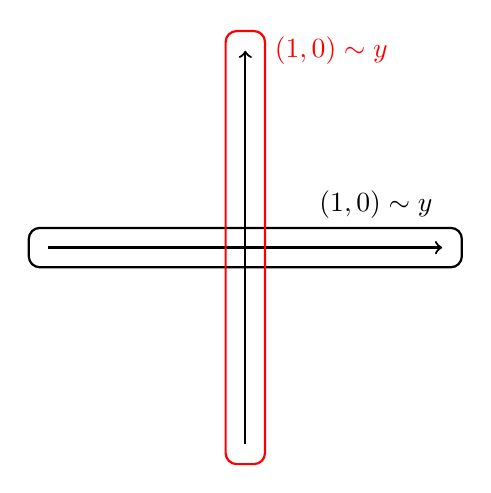
\begin{tikzpicture}[scale=2.5]
				\draw[thick, ->] (-1,0) -- (1,0);
				\draw[thick, ->] (0,-1) -- (0,1);
				\draw[thick, rounded corners] (-1.1,-0.1) rectangle (1.1,0.1);
				\draw (1,0.1) node[anchor=south east] {$(1,0)\sim y$};
				\draw[thick, red,rounded corners] (-0.1,-1.1) rectangle (0.1,1.1);
				\draw[red] (0.1,1) node[anchor=west] {$(1,0)\sim y$};5
			\end{tikzpicture}
		\end{center}
		\item Ja.
		\item Nein. $(1,0)\sim (0,0), (0,1)\sim (0,0)$, aber $(1,0)\sim (0,1)$ stimmt nicht.
	\end{parts}
\end{proof}
\end{document}
